\documentclass{article}

\usepackage{tikz}
% to allow storage of figure 
\usetikzlibrary{external}
\tikzexternalize[prefix=figures-to-import/]
\usetikzlibrary{bayesnet}

\begin{document}

Note: This document must be run with shell: pdflatex -shell-escape

\tikzset{external/force remake}
\tikzsetnextfilename{ASP-graphical-model}
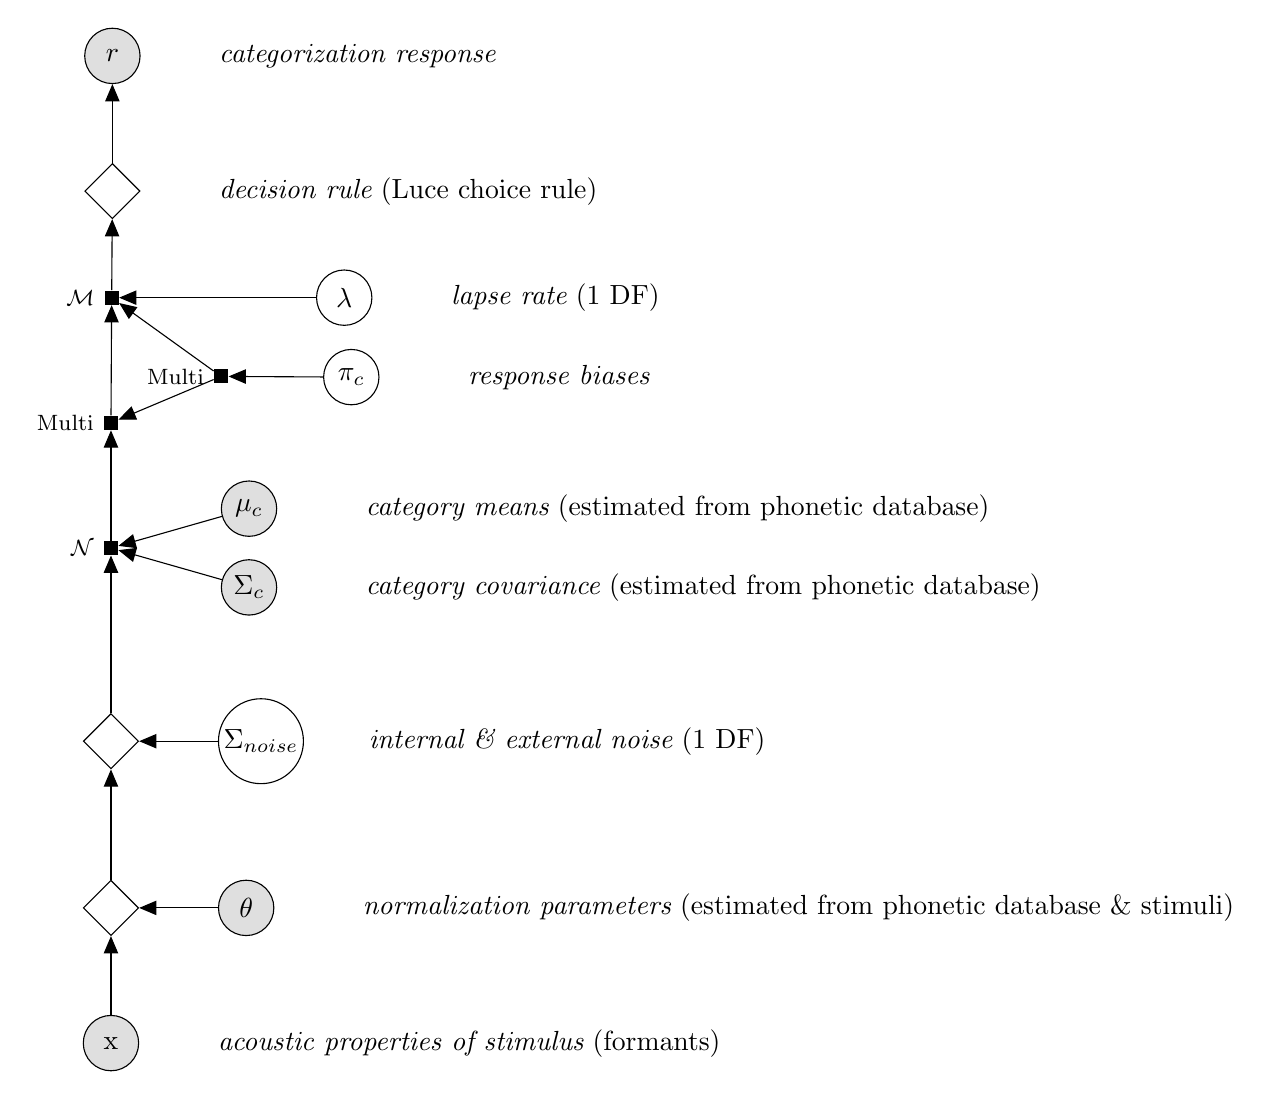
\begin{tikzpicture}
    \node[obs] (r) {$r$} ; %
    \node[const, right=of r, xshift=-.009cm] (r_description) {{\em categorization response}} ; %
    \node[det, below=of r] (decision) {} ; %
% decisions
    \node[const, right=of decision, xshift=-.009cm] (decision_rule) {{\em decision rule} (Luce choice rule)} ; %
    \factor[below=of decision, xshift=-.009cm, yshift=-.5cm] {response-dist} {left: $\mathcal{M}$} {} {}; %
    \factor[right=of response-dist, xshift=.8cm, yshift=-1cm] {prior-dist} {left: Multi} {} {}; %
    \factor[below=of response-dist, xshift=-.009cm, yshift=-1cm] {multi} {left: Multi} {} {}; %
    \node[latent, right=of response-dist, xshift=1.5cm] (l) {$\lambda$} ; %
    \node[const, right=of l, xshift=-.009cm] (lapse) {{\em lapse rate} ($1$ DF)} ; %
    \node[latent, right=of prior-dist, xshift=.2cm, yshift=-.009cm] (pi_n) {$\pi_{c}$} ; %
    \node[right=of pi_n] (beta_description) {{\em response biases}} ;
% edges
    \edge {decision} {r} ;
    \edge {response-dist} {decision} ; %
    \edge {multi} {response-dist} ; %
    \edge {prior-dist} {response-dist} ; %
    \edge {prior-dist} {multi} ; %
    \edge {l} {response-dist} ; %
    \edge {pi_n} {prior-dist} ;
% representations
    \factor[below=of multi,  yshift=-1cm] {x_prime} {left:$\mathcal{N}$} {} {}; %
     %\node[above=of x_prime] (dots) {$\vdots$} ; %
    \node[obs, right=of x_prime, yshift=.5cm, xshift=.3cm] (mu_n) {$\mu_{c}$} ; %
    \node[obs, right=of x_prime, yshift=-.5cm, xshift=.3cm] (sigma_n) {$\Sigma_{c}$} ; %
    \node[right=of mu_n] (mu_n_description) {{\em category means} (estimated from phonetic database)} ;
    \node[right=of sigma_n] (sigma_n_description) {{\em category covariance} (estimated from phonetic database)} ;

% edges
    \edge {x_prime} {multi} ; %
    \edge {mu_n} {x_prime} ; %
    \edge {sigma_n} {x_prime} ; %
% noise
    \node[det, below=of x_prime, yshift=-1cm] (x_prime2) {} ; %
      %\node[above=of x_prime2] (dots) {$\vdots$} ; %
    \node[latent, right=of x_prime2] (sigma_noise) {$\Sigma_{noise}$} ; %
    \node[right=of sigma_noise, xshift=-.3cm] (sigma_noise_description) {{\em internal \& external noise} (1 DF)} ;
%edges
    \edge {x_prime2} {x_prime} ; %
    \edge {sigma_noise} {x_prime2} ; %
% normalization
    \node[det, below=of x_prime2, yshift=-.4cm] (x_prime3) {} ; %
    \node[obs, right=of x_prime3] (theta) {$\theta$} ; %
    \node[right=of theta] (theta_description) {{\em normalization parameters} (estimated from phonetic database \& stimuli)} ; %
    \node[obs, below=of x_prime3] (x) {x} ; %
    \node[const, right=of x, xshift=-.009cm] (x_description) {{\em acoustic properties of stimulus} (formants)} ;
%edges
    \edge {x_prime3} {x_prime2} ; %
    \edge {theta} {x_prime3} ; %
    \edge {x} {x_prime3} ; %
\end{tikzpicture}

\end{document}